\subsection{The DOM} % (fold)
\label{sub:dom}

Apart from the native capabilities of the \idx{JavaScript} language, browsers provide a very useful tool to deal with the \ida{HTML} elements of the page, the \ida{DOM}.
It consists of an \ida{API} accessible from \idx{JavaScript} and it allows the dynamic retrieval, creation, modification and deletion of \ida{HTML} elements within the page scope.

This \ida{DOM} is a fully object-oriented representation of the web page, in which every element is depicted as an object with properties that responds accordingly to different methods.
Those properties determine the document structure, style and content.
Actually, this representation is not bound to \idx{JavaScript} or even browsers, it can be accessed with other programming languages and applications.
But since \idx{JavaScript} is the most popular one in browsers they are usually delineated as partners.

The basic idea behind the \ida{DOM} is that the page is composed around a tree of elements (nodes).
Starting from the root node, every element may have an indeterminate number of children.
The \ida{DOM} provides some methods to traverse that tree either by depth (between a parent and its children) or breadth (between siblings).
Visually, children are drawn inside their parent bounds, but that behavior can be subverted with the use of \ida{CSS} properties.

This \ida{API} forms a standalone standard maintained by the \ida{W3C}.
But, as other web standards, its support varies from browser to browser, each one suffering from either partial implementations, vendor extensions or, commonly, both.

Another chronic burden is that modifying visible elements in the page is a very expensive operation.
Since the \ida{DOM} is linked to the visual representation of the page, every modification triggers a live partial or full page reflow.
For this reason it is advisable that, when several \ida{DOM} changes are needed, they are made on a detached element and, at the end, that element is attached to the \ida{DOM} tree.

\subsubsection{DOM Objects} % (fold)
\label{ssub:domobjects}

There are several objects available to \idx{JavaScript} exposed by the \ida{DOM}.
Those objects properties and functions conforms the \ida{API}.
The most important ones are:

\begin{description}
  \item[window] This object represents the browser window itself, and it allows the retrieval and modification of several properties related to the browser in general and the document window in particular.
  Since this is the global object, all of its properties are initially accessible with no need to specify \texttt{window}, as if they were \emph{local variables}, so for example \texttt{location} is the same as \texttt{window.location}.
  It has lots of attributes, some of the most important being:
  \begin{description}
    \item[window.location] Through this property the location (\ida{URL}) for the window can be accessed and modified.
    \item[window.innerHeight / window.innerWidth] These readonly properties contains the size of the content area of the browser window. That is, only the area occupied by the document, not counting external browser elements like the title bar, the status bar or the menu bar.
    \item[window.screen] This object describes the screen: its size, its color depth and the position of the window in the screen.
    \item[window.navigator] This object contains information about the browser, such as the user agent, browser version, platform, language, plugins installed, etc.
    Modern browsers also include access to geolocation data in this object.
    \item[window.history] This object provides an interface for manipulating the browser session history, i.e., the pages visited by the user in this tab.
    Initially it was not possible to change or read the history, only traveling through it, but an \ida{HTML}5 extension encloses several methods to add and modify history entries (but not read).
    \item[window.localStorage] This object contains the Web Storage \ida{API}, one of the key components of \ida{HTML}5.
    Basically, it simplifies the storage of significant amounts of data locally in the browser, so that it is available in successive visits using a key/value pairs interface.
    \item[window.applicationCache] Another key component of \ida{HTML}5, through this object the cache of static files is managed, allowing the rising of offline web applications.
    \item[window.setTimeout() / window.clearTimeout()] This useful function executes a function after the specified delay.
    It returns a timer identifier that allows canceling it afterwards.
    \item[window.setInterval() / window.clearInterval()] Similar to the previous function, this sets a timer that will repeatedly execute a function with a fixed time delay between calls.
    \item[window.open()] It opens an additional window with the size and properties specified.
    \item[window.close()] It closes the current window but it only works if the window was opened programmatically by \idx{JavaScript}.
    \item[window.scroll()] This function scrolls the window to a particular coordinate in the document.
    \item[window.resizeTo()] This function dynamically resizes the window.
    \item[window.escape() / window.unescape()] A very useful utility function to encode/decode special characters in a string so it is suitable for cookie storage or \ida{HTTP} requests.
  \end{description}
  \item[document] The interface of this object comprises all the necessary tools to retrieve and modify the document, with particularly valuable functions for \ida{DOM} retrieval.
  Therefore, it is almost impossible to make a web application without accessing this object, either directly or employing a \idx{JavaScript} library.
  The most relevant properties and methods are:
  \begin{description}
    \item[document.cookie] This object contains the interface to get and set the cookies of a page, that is, a small amount of data stored in the client that will be usually to maintain a session with the server.
    Since these cookies will be transferred with every request to the server, its overuse could slow the page loading.
    \item[document.styleSheets] This readonly object contains references to all the stylesheets in the page.
    There are also properties for accessing other kind of elements, like \texttt{document.links}, \texttt{document.images}, \texttt{document.forms}, etc, but in modern \idx{JavaScript} paradigms these are not very used anymore.
    \item[document.title] This object gets and sets the title of the document, which most browsers used for their window titles.
    \item[document.referrer] This string contains the address of the page that linked to this page.
    \item[document.getElementById()] This function returns the element with the specified id.
    It is the basic pillar of element manipulation, since it is the most used method to directly fetch an element.
    Because of that, multiple libraries have wrapped this function under the \texttt{\$()} short name.
    \item[document.getElementsByClassName()] Similar to the previous function, this one returns the elements with the given class name.
    This is natively implemented only in relatively modern browsers, but it is so obviously useful that it was already widely implemented in most third-party libraries and toolkits.
    \item[document.getElementsByTagName()] The third-wheel of the last two functions, this one returns the elements with the given tag name.
    It seems useful for dealing with all the elements of a certain type, but since \ida{DOM} manipulations are normally needed inside a certain document \emph{block} rather than across element types in all the document, its counterpart that affects only an element children is more interesting.
    \item[document.createElement()] This function returns a newly created element with the given tag name.
    This does not add the element to the document tree, it is needed to insert it manually later on.
    \item[document.createAttributeName()] This function returns a newly created attributed node with the given name.
    This function does not add the attribute to any element, it is needed to set it manually later on.
    This is not very used, since the \texttt{element.setAttributeName()} is more convenient, but it could be more efficient if the same attributes need to be changed in a lot of different elements.
    \item[document.createDocumentFragment()] This function creates a document fragment, an temporary holding object designed to store nodes before adding them to the document.
    It is not very known, but it is one of the best performance-wise solutions when several elements need to be added to the document.
    \item[document.evaluate() / document.createExpression()] These functions provide an interface to work with \idx{XPath} expressions.
    These advanced expressions enable complex and precise selections of element nodes in the document tree.
    Regrettably, only some browsers support this powerful mechanism.
    \item[document.querySelector() / document.querySelectorAll()] These functions allows the retrieval of elements using the well known \ida{CSS} selectors.
    The difference between the two functions if that the former returns only the first matched element and the latter returns all the matched elements.
    It is only supported by very modern browsers, but it appears to have a bright future because of its ease of use and familiarity.
  \end{description}
  \item[element] Once an element is retrieved or created using the \ida{DOM}, the returned object conforms to the \texttt{element} interface.
  This interface details all the actual properties to modify not only the \ida{DOM} structure, but the style and content of that certain element.
  \begin{description}
    \item[element.parentNode] Returns the parent node of this element.
    \item[element.childNodes] Lists all the child nodes of this element.
    \item[element.nextSibling] Retrieves the node immediately following this one in the document tree.
    \item[element.previousSibling] Retrieves the node immediately preceding this one in the document tree.
    \item[element.attributes] Arranges all the attributes of this element.
    \item[element.id] Sets and gets the id attribute of the element.
    \item[element.className] Sets and gets the class attribute of the element.
    \item[element.clientHeight / element.clientWidth] Returns the element size, counting the padding but not the border.
    \item[element.offsetHeight / element.offsetWidth] Returns the element size, counting both the padding and the border.
    \item[element.offsetLeft / element.offsetTop] Returns the distances from the left/top border to the \texttt{offsetParent}'s node.
    \item[element.offsetParent] This is the parent node from which all offset calculations are currently computed.
    Depending on \idx{CSS} properties, it could be the immediate parent node or other ancestor.
    \item[element.innerHTML] Sets and gets the content of the element as a string with HTML markup, quite useful and convenient.
    It is one of the fastest ways of modifying the \ida{DOM}, since this task is basically the same one browser engines carry out when rendering an \ida{HTML} page; therefore it is very optimized.
    \item[element.contentEditable] Another nice addition in \ida{HTML}5, it toggles the ``editable'' property of an element.
    When this is active, the user can edit the element like in a \idx{WYSIWYG} editor (without any format buttons, just the content).
    \item[element.style] This object maps (almost) all the \ida{CSS} properties relevant to this element, so they can be directly consulted or altered.
    \item[element.appendChild() / element.removeChild()] Insert/delete the given node as the last child of this element.
    \item[element.insertBefore()] Insert the first given node as a child of this element, just before the second given node (that is also a child node).
    \item[element.getAttribute() / element.setAttribute() / removeAttribute()] Gets/sets/deletes an attribute of this element.
    \item[element.addEventListener()] This function attaches an event listener, that is, a function that will be called when that kind of event occurs in this element.
  \end{description}
  \item[event] Since \idx{JavaScript} is designed to control the document behavior, the specification provides a powerful interface to manage events.
  These events are not usually created by the programmer, the common flow is that the browser generates them when a certain action happens and then the programmer should handle them.
  There are events linked to user actions like mouse clicks or key strokes, but there are also events dealing with automatic \ida{API}s like \ida{HTML}5 storage.
  \begin{description}
    \item[event.clientX / event.clientY] The coordinates associated with the event, useful for knowing the exact position of the mouse in mouse-triggered events.
    \item[event.charCode] The code of the key pressed, if the event is a key press event.
    \item[event.preventDefault()] Most events have a default action that the browser will trigger; this method cancels that action.
    For example, if the user clicked a link the browser will follow the anchor, but if we catch the event and call this method, the browser will not do anything.
    \item[event.stopPropagation()] By default, events are propagated from the specific element to the top element in the \ida{DOM} tree, notifying every parent handlers in that way.
    This method stops that propagation so that those handlers are not notified.
    It is a common mistake to assume that these two last methods are equivalent, but their effects are mutually exclusive.
  \end{description}
\end{description}

\begin{figure}[htbp]
  \centering
    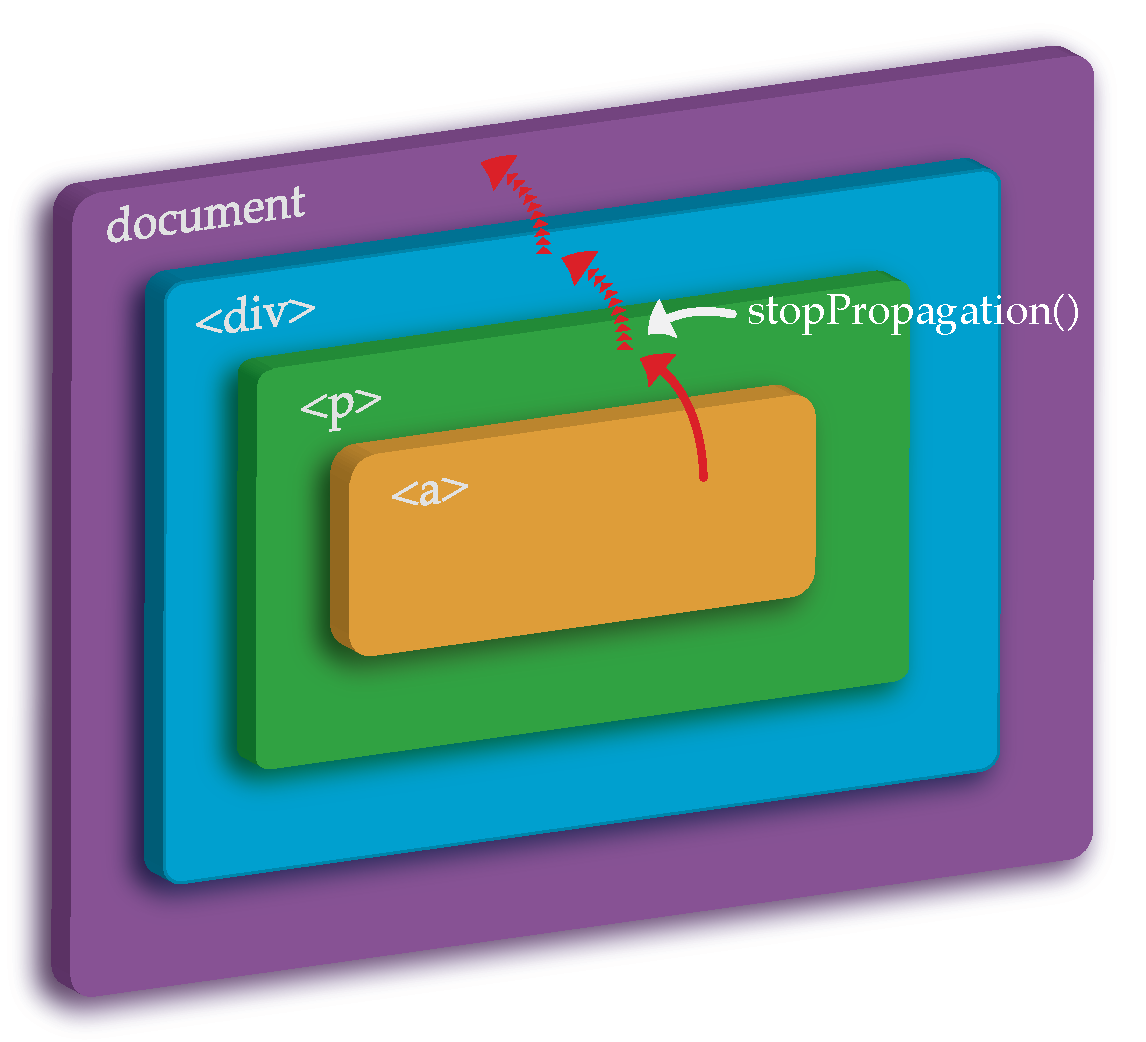
\includegraphics[width=\textwidth]{dom-event-bubbling}
  \caption[DOM event propagation]{DOM event propagation and the effect of stopPropagation()}
  \label{fig:dom-event}
\end{figure}

% subsubsection domobjects (end)

% subsection dom (end)